\chapter{Newton's Laws}

\section{Dynamics}

Newton's Laws provide the framework for the dynamics of classical particle motion.

Question of Classical Mechanics:

\begin{center}
	\textit{Given $\vec r_0$ and $\vec v_0$ of the particle, with mass $m$, determine its subsequent motion, $\vec r(t)$, for all time $t$.}
\end{center}

\subsection{Within Context}

Newton originally formulated the laws to solve the question of gravity -- along the way, he formulated concepts like forces and momentum.

\section{Newton's Laws}

\begin{definition}[Newton's Laws]
	The three laws of motion:

	\begin{description}
		\item[Law of Invertia] A particle remains at rest or moving with constant velocity unless influenced by a force.
		\item[$\mathbf{F = m a}$] The change in a particle's motion (i.e. its acceleration) is proportional to the force impressed, as vectors. 
		\item[Action / Reaction] Forces come in pairs: to every action by one particle on another, there is an equal and opposite force in return. 
	\end{description}
\end{definition}

\subsection{First Law}

There exist \textit{intertial frames of reference}, that is, a frame in which a \textit{free particle}\footnote{particle subject to absolutely no influences} has constant velocity.

\begin{remark}
	Essentially, a frame at rest and a frame with constant velocity are the same.
\end{remark}

Mathematically, this is expressed as

\begin{equation}
	\frac{\D^2 \vec r}{\D^2 t} = 0
\end{equation}

\subsection{Second Law}

Denote the force by $\vec F$

Two different particels subject to the same force (e.g. a spring). After the unfluence of the force (e.g. left spring), particle 1 has speed $v_1$ and particle 2 has speed $v_2$.

Consider the ratio

\begin{equation}
	\frac{v_1}{v_2} \equiv \frac{m_2}{m_1}
\end{equation}

where $m_i$ is an intrinsic property of the $i$-th particle we call its mass [unit: kg].

\textit{Assumption:} $m$ is independent of $\vec F$ and $\vec v$.

So we can write a relation:

\begin{equation}
	m_1 v_1 = m_2 v_2
\end{equation}

Assume we start from rest and apply some force for some duration, then we have

\begin{equation}
	m_1 \Delta v_1 = m_2 \Delta v_2 = F \Delta t
\end{equation}

And thus we have

\begin{equation} \label{eq:force-mv}
	F \Delta t = m \Delta v \implies F = \frac{m \Delta v}{\Delta t} = \frac{\Delta (mv)}{\Delta t} 
\end{equation}

\begin{definition}
	Define the (physical) \textbf{momentum} of a particle to be

	\begin{equation}
		\vec p = m \vec v
	\end{equation}
\end{definition}

As so we have with \cref*{eq:force-mv} the following

\begin{equation}
	\vec F = \frac{\Delta \vec p}{\Delta t}
\end{equation}

\begin{enumerate}
	\item As $\Delta t \to 0$, we have that
	
	\begin{equation}
		\vec F = \frac{\D \vec p}{\D t}
	\end{equation}

	\item Forces (empirical) obey the \textit{principle of superposition}.

	\begin{equation}
		\vec F_\mathrm{net} = \sum_i \vec F_i
	\end{equation}
\end{enumerate}

Altogether we have that

\begin{equation}
	\vec F_\mathrm{net} = \frac{\D \vec p}{\D t}
\end{equation}

If $m$ is constant, then we have

\begin{equation}
	\frac{\D \vec p}{\D t} = m \frac{\D \vec v}{\D t} = m \vec a \implies \boxed{\vec F_\mathrm{net} = m \vec a}
\end{equation}

mass is a measure of an object's inertia -- \textit{tendency to persist in its state of motion}.

\subsection{Third Law}

\begin{definition}
	A force is a directed influence between pairs of particles.
\end{definition}

If force of 1 on 2 is $\vec F_{12}$,

then force of 2 on 1 is $\vec F_{21} = - \vec F_{12}$.

\textbf{IMPORTANT:} Forces always come in pairs! (e.g. When we are sitting on our seats, its us pushing on the seat, and the seat pushing on us. The force of us pushing on the seat comes from gravity.)

\begin{example}
	Given $\vec r_0$, $\vec v_0$, and $m$, fint $\vec r(t)$

	Newton's laws:

	\begin{enumerate}
		\item go to an intertial frame: $\vec r(t)$
		\item Identify forces acting on particle: $\vec F$
		\item Then we just solve the differential equation.
		
		\begin{equation}
			\vec F_\mathrm{net} = m\frac{\D^2 \vec r}{\D t^2}
		\end{equation}

		Our initial conditions are the two givens.
	\end{enumerate}
\end{example}

\section{Forces}

There are two types of forces:

\begin{enumerate}
	\item Contact forces
	\item Long range forces
\end{enumerate}

\subsection{Contact Forces}
arises due to contact between bodies.

Deconstruct the force into components parallel and perpendicular to the surface of contact.

\begin{itemize}
	\item The component $\perp$ is called the \textbf{normal force}, $\vec F_N$.
	\item The component $\parallel$ is called the \textbf{frictional force}, $\vec F_f$.
\end{itemize}

\begin{remark}
	Normal forces are constraint\footnote{They generally constraint the motion rather than ``generating'' the motion.} forces.
\end{remark}

\subsection{Tension Forces}

arise due to internal elastic forces of a one-dimensional string (rope / chain / etc.)

An ideal massless string has a uniform tension force throughout. (Otherwise parts of the string can have infinite acceleration.)

\begin{remark}
	If any body is considered to be massless, we assume automatically $F_\mathrm{NET} = 0$ for that body. 
\end{remark}

The direction of the force is:

\begin{itemize}
	\item Directed away from the string for the string
	\item Directed away from the body if the string is attached to some
\end{itemize}

\subsection{Long-Range Forces}

Forces exerted over a distance between bodies not in contact.

e.g. gravity, electromagnetic, (strong nuclear, weak nuclear)

\begin{itemize}
	\item \textbf{Weight} $\vec F_g = -mg$ downward -- the downward force exerted by a body near earth's surface.

	\begin{remark}
		Why does the specific force $F_g$ involved $m$, when $m$ is part of the 2nd law and independent of forces?

		Perhaps, $F_g = m_g g$, then free fall means $m_g g = m_I a = m_I g$ which means

		\begin{equation}
			m_g = m_I
		\end{equation}

		The above is called the \textbf{Principle of Equivalence}
	\end{remark}
\end{itemize}

\subsection{Friction}

Component of contact force parallel to surface of contact.

Based on experiment, friction has two behaviors:

\begin{itemize}
	\item \textbf{Static} -- when \textit{no} relative motion between objects in contact. Acts to balance forces to ensure constant relative velocity. Has max value.
	\item \textbf{Kinetic} -- \textit{is} relative motion between objects in contact. Acts in opposition to relative motion (i.e. to decelerate the object). Constant in magnitude (independent of relative speed \& surface area).
\end{itemize}

The phenomenological models are:

\textbf{Static Friction}

\begin{equation}
	F_{f_s} \leq \mu_s F_N
\end{equation}

\begin{itemize}
	\item $\mu_s$ is coefficient of static friction.
	\item $F_N$ is between the objects in contact.
\end{itemize}

\begin{equation}
	F_{f_k} = \mu_k F_N
\end{equation}

\begin{itemize}
	\item $\mu_k$ is coefficient of kinetic friction
	\item $F_N$ is between the objects in contact.
\end{itemize}

\begin{remark}
	Generally, $\mu_s \geq \mu_k$.
\end{remark}

\subsection{Comments}

These forces are \textit{phenomenological} in character.

That is, models based on empirical observation disregarding their fundamental origin.

However, so far as we know, there are only 4 fundamental forces in nature:

\begin{itemize}
	\item Gravity
	\item Electromagnetic
	\item Strong Nuclear
	\item Weak Nuclear
\end{itemize}

All these 4 forces are long range and position dependent.

\section{Scenarios of Newton's Laws}

\subsection{Constant Forces}

\subsection{Variable Forces with Time}

\subsection{Variable Forces with Position}

\subsection{Variable Forces with Velocity}

\section{Algorithm for Solving Constant-Force Newton's Laws Problems}

\begin{enumerate}[1)]
	\item Isolate relevant bodies for analysis
	\item For each body in 1), draw a free body diagram (FBD) which includes
	
	\begin{enumerate}[(a)]
		\item \textit{all} forces acting on body (may on occassion ignore some forces)
		\item an inertial coordinate system for analysis
	\end{enumerate}
	\item Write down the equations of motion for each body in 1) using the FBD in 2); i.e. write Newton's 2nd Law in component form.
	\item Impose any kinematic constraints on the bodies in your equations from 3), along with Newton's 3rd law relation.
	\item Solve for desired unknowns. Treat the equations from 4) as a system of algebraic equations, regardless of the origin.
\end{enumerate}

\section{Pulleys}

Mechanical device used to redirect tension forces. An ideal pulley is massless and frictionless. If pulley doesn't rotate, then $F_{T_1} = F_{T_2}$. Redirects $F_T$. If they are not equal, the pulley rotates.

\section{Newton's Laws in Polar Coordinates}

%! TODO
\section{Simple Harmonic Motion}

\begin{figure}[H]
	\centering
	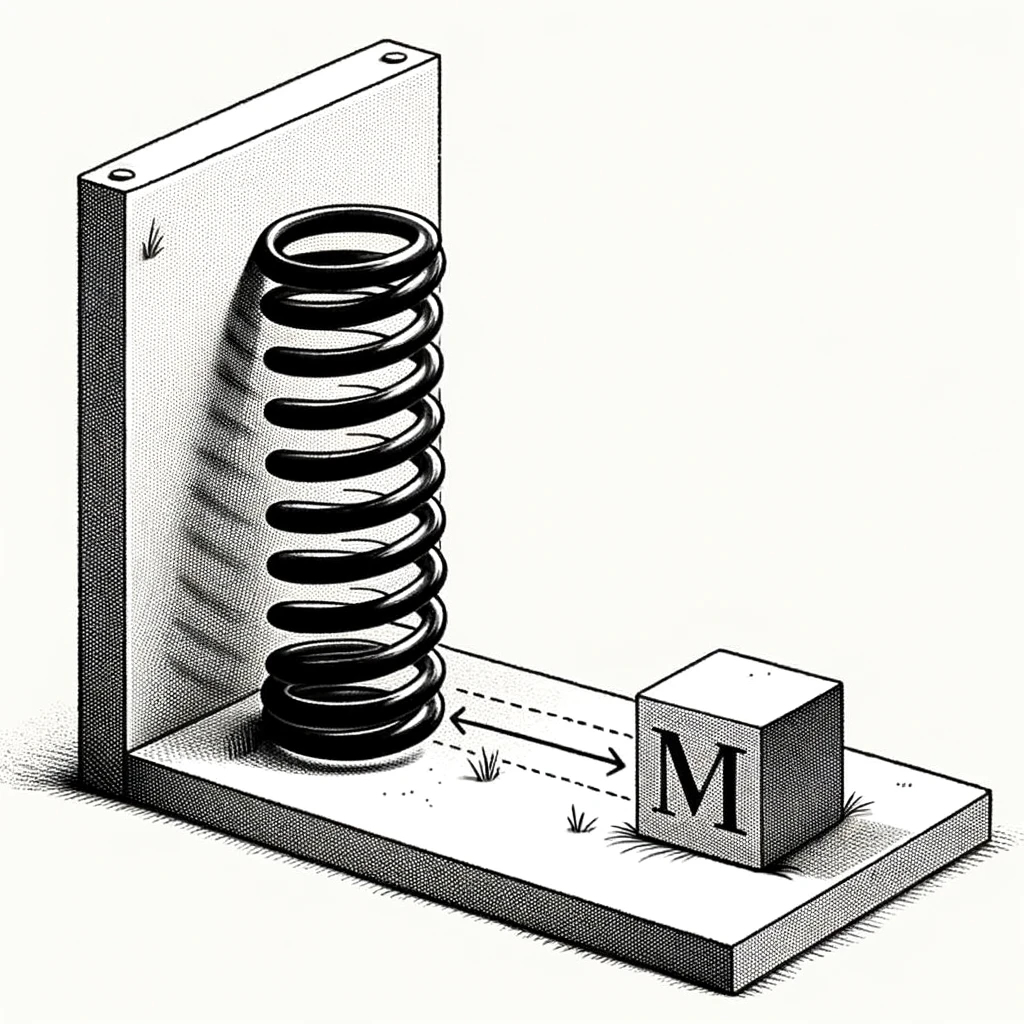
\includegraphics[width=0.5\linewidth]{assets/spring2wall.jpg}
	\caption{DALLE is Smart}
\end{figure}
A spring (massless) exerts a linear restoring force, $\vec F_s$, given by (Hooke's Law):

\begin{equation}
	\vec F_S = - k \Delta \vec r
\end{equation}

where $k$ is the spring constant ($\si{\N\m}$) and $\Delta \vec r$ is displacement of spring from equilibrium length.

\begin{example}
	We have a block of mass $M$ connected to a wall by a spring of constant $k$.
\end{example}

If we setup Newton's second law:

\begin{equation}
	\sum F = ma \implies -kx = m \ddot x
\end{equation}

Let $\omega \equiv \sqrt{\frac{k}{m}}$, the this equation is 

\begin{equation}
	\boxed{\ddot x = -\omega^2 x}
\end{equation}

Our guess ansatz for the solution:

\begin{equation} \label{eq:shm-general-sol}
	x(t) = c_1 \cos(\omega t) + c_2 \sin(\omega t)
\end{equation}

Aside: Euler identity $e^{i\theta} = \cos\theta + i\sin\theta$ allows us to construct complex solutions

\begin{equation}
	\tilde{x} = \tilde{c}_1 e^{i\alpha t} + \tilde{c}_2 e^{i\beta t}
\end{equation}

If we have initial conditions $x(0) = x_0$ and $\dot x(0) = 0$, then we have:

\begin{equation}
	x(t) = x_0\cos(\omega t)
\end{equation}

\begin{example}
	We have a mass $m$ hung from the ceiling by a spring with spring constant $k$.
\end{example}

\begin{sol}
	CHECK TABLET FILL
\end{sol}

We have $\cos(\theta + 2\pi) = \cos(\theta)$,

here, $\cos(\omega t + 2 \pi) = \cos(\omega t)$

let $t = t_0 - T$

\begin{align}
	\cos(\omega t_0 - \omega T + 2\pi) &= \cos(\omega t_0)\\
	\omega T - 2\pi &= 0\\
	T &= \frac{2\pi}{\omega}
\end{align}

$T$ is the \textbf{period}: time to complete one oscillation.

Then, $T = \frac{2\pi}{\omega}$

$f$ is the \textbf{frequency}, $f \equiv \frac{1}{T}$: number of oscillations per unit time ($[f] = s^{-1} \equiv \si{\Hz}$)

\begin{equation}
	\omega = 2\pi f
\end{equation}

One is angular, one is frequency.

\begin{example}
	The pendulum
\end{example}

\begin{sol}
	CHECK TABLET
	%! TODO
\end{sol}